\section{Background}\label{sec:vuln_background}

This section establishes the terminology used in this paper and gives an
overview of the terminology used in other works.

\subsection{Glossary}

This section briefly explains terms used in the SIBAS G programming language.

\paragraph{Program} The complete SIBAS program that can be compiled and uploaded to run cyclical on its device. It is hierarchic ordered into function packages.

\paragraph{Function Package} A function package describes a broader functionality of a component, e.g. the parking brake, and consists of multiple function groups.

\paragraph{Function Group} Function groups are the smallest part of the program hierarchy. They can either contain multiple function groups or models describing the software. The model itself consists of two entities: function blocks and signals.

\paragraph{Function Block} Function blocks are predefined methods that can take multiple inputs and have multiple outputs.

\paragraph{Signal} The variables of the program are projected as signals. Visually they are either represented by a flag when they don't origin in the current function group or otherwise as a line between two function blocks. There are different types of signals. For this context most importantly, global signals and local signals. Global signals origin from another function package or are created to be read from different function packages. They are only allowed to be written to by one actor and can be identified by an '\$' in front of the signal name. Local variables are only write and readable from the same function package. 

\paragraph{Function ID} Function IDs are unique identifiers that are assigned by the developer to function groups that implement a common function. A function ID consists of at least one function group, though more complex functions are spread over multiple IDs.

\subsection{SIBAS Control Technology}

SIBAS 32, the successor of SIBAS 16, is a control technology used in trains. Its goal is to provide a common interface between different components, e.g. central control device or brake control device. SIBAS 16 was first introduced in 1983 and was further developed until in 1992 SIBAS 32 was released. The software that runs SIBAS is projected in an editor called SIBAS G in a model-based approach. The model translates automatically into C code and eventually compiles to run as intended on embedded systems. Every function block is validated before being allowed to use, hence when testing the software, only the logic of the software needs to be tested.


\subsection{SAMAPI - Sibas Application Model API Specification}

SAMAPI provides the possibility to read or create SIBAS models.
It is written in Java but is distributed to use in Python 2.7 via Jython\footnote{\url{http://www.jython.org/docs/index.html}}.

\begin{figure}[ht]
	\centering
	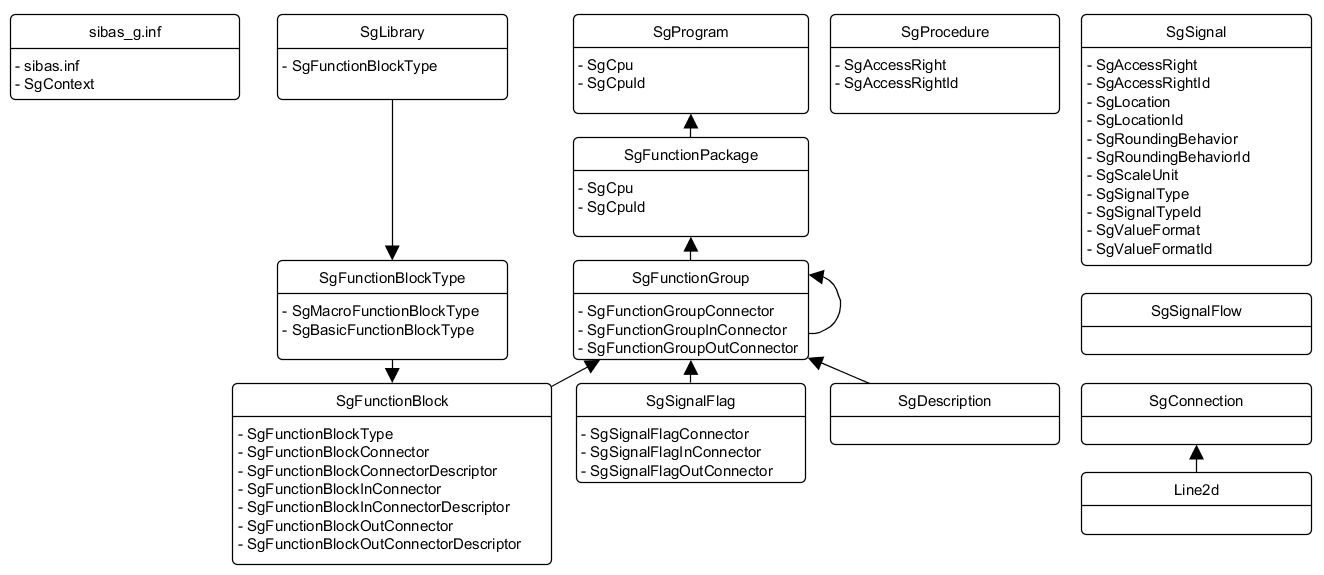
\includegraphics[width=1\textwidth]{graphic/samapi_classes.png}
	\caption{SAMAPI - Class Overview}
	\label{fig:samapi}
\end{figure}

\autoref{fig:samapi} describes the structure of the API. First, either a function package file or a program file has to be loaded, returning a SgFunctionPackage or SgProgram object respectively. On this object several methods can be called, e.g. 'getFunctionBlocks' or 'getFunctionGroups', returning a set of specified objects. Whenever calling a function on an object, ot only returns objects that are in its context.



